\documentclass[border=5pt]{standalone}
\usepackage{tikz}
\usepackage{tikz-3dplot}
\usetikzlibrary{arrows.meta, 3d, perspective, calc}
\usepackage{amsmath}
\begin{document}
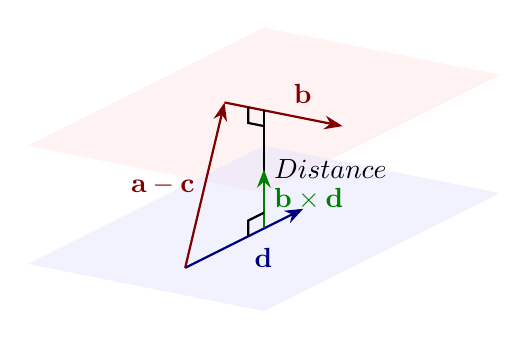
\begin{tikzpicture}[>=Stealth, x={(1cm,0.5cm)}, y={(0cm,1cm)}, z={(1cm,-0.2cm)}]

    % Planes
    \fill[red!10, opacity=0.5] (0,1.5,0) -- (3,1.5,0) -- (3,1.5,3) -- (0,1.5,3) -- cycle;
    \fill[blue!10, opacity=0.5] (0,0,0) -- (3,0,0) -- (3,0,3) -- (0,0,3) -- cycle;

    % Normals
    \draw[->, thick, red!50!black] (1.5,1.5,1) -- node[above right] {$\mathbf{b}$} (1.5,1.5,2.5);
    \draw[->, thick, blue!50!black] (0.5,0,1.5) -- node[below right] {$\mathbf{d}$} (2,0,1.5);

    \draw[->, thick, red!50!black] (0.5,0,1.5) -- node[midway, left] {$\mathbf{a}-\mathbf{c}$} (1.5,1.5,1);

    \draw[thick] (1.5,0,1.5) -- node[midway, right] {$Distance$} (1.5,1.5,1.5);

    \draw[->, thick, green!50!black] (1.5,0,1.5) -- node[midway, right] {$\mathbf{b} \times \mathbf{d}$} (1.5,0.75,1.5);

    \draw[thick] (1.3,0,1.5) --(1.3,0.2,1.5)--(1.5,0.2,1.5);

    \draw[thick] (1.5,1.5,1.3) --(1.5,1.3,1.3)--(1.5,1.3,1.5);
\end{tikzpicture}
\end{document}
